\documentclass[11pt,a4paper]{article}

\usepackage{kotex}
\usepackage{amsmath,amssymb,amsfonts,amsthm,bm}
\usepackage{graphicx}
\usepackage[labelfont=bf,labelsep=space]{caption}
\captionsetup[figure]{name=Fig.}
\usepackage{pgfplots}
\pgfplotsset{compat=1.18}
% RdBu_r diverging colormap (ColorBrewer): blue=low (good) -> white -> red=high (bad),
% matching the v_ss contour colorscale used in the interactive HTML figures.
\pgfplotsset{
  colormap={RdBu_r}{
    rgb255=(5,48,97) rgb255=(33,102,172) rgb255=(67,147,195) rgb255=(146,197,222)
    rgb255=(209,229,240) rgb255=(247,247,247) rgb255=(253,219,199) rgb255=(244,165,130)
    rgb255=(214,96,77) rgb255=(178,24,43) rgb255=(103,0,31)
  }
}
\usetikzlibrary{arrows.meta, calc, positioning, decorations.pathreplacing, patterns, shapes.geometric}
\usepackage{booktabs}
\usepackage{algorithm}
\usepackage{algpseudocode}
\usepackage{float}
\usepackage[numbers,sort&compress]{natbib}
\usepackage{hyperref}
\usepackage{geometry}
\geometry{margin=25mm}

\title{Support Flow Tensor Field for Fast Build-Orientation Candidate Generation in Support-Requiring Additive Manufacturing}
\author{}
\date{}
% WORDCOUNT: 3883 words by pandoc plain export (main manuscript, 2026-06-26).

\newtheorem{definition}{Definition}
\newtheorem{theorem}{Theorem}
\newtheorem{proposition}{Proposition}
\providecommand{\bibcommenthead}{}

\begin{document}

\maketitle

\begin{abstract}
Build orientation strongly controls support volume in additive manufacturing, but exhaustive orientation sweeps remain costly.
The proposed method targets support-requiring additive-manufacturing processes in which build orientation changes the amount of removable support material; it is not intended for inherently support-free processes.
This paper proposes the Support Flow Tensor Field (SFTF), a fast candidate generator that ranks promising build directions before local verification by a support-volume grid or slicer.
For each sampled direction, SFTF casts rays from overhang faces to actual receiver faces and forms a direction-dependent asymmetric flow tensor.
The build-plate support term is further interpreted as a virtual ground receiver, making the dominant predictive term a unified Rayleigh cost.
On five organic freeform benchmark meshes with a $1^\circ$ tomography grid, verifying the $\pm 10^\circ$ neighborhoods of the top-20 SFTF candidates uses $3.40\%$ of the grid on average and obtains a mean support-volume ratio of $1.14$ with maximum $1.66$; on these meshes the tensor features $B$ and $\tilde R=R+B$ are the most stable single predictors of the tomographic support volume (mean Spearman $0.59$ and $0.61$).
The paper also introduces Adaptive Verification Escalation (AVE), an automatic hard-case escalation rule based on local-verification confidence signals; on a five-group cached $1^\circ$ audit of $21$ ratio-valid records it keeps every record below ratio $2.0$ (mean $1.14$, maximum $1.93$) at a mean budget of $13.94\%$.
We also report a clear limitation: on large mechanical parts (up to $1.04$M faces) the tensor features do not predict support volume, and at a matched budget a simple uniform-axis window seeding outperforms the SFTF ranking, so SFTF is best positioned as an interpretable warm start for organic parts rather than a general replacement for broad coverage.
These results show that SFTF is best viewed not as a replacement for precise support-volume optimization, but as a low-cost warm start that concentrates expensive verification on a small number of likely basins.
\end{abstract}

\noindent\textbf{Keywords:} Support Flow Tensor Field (SFTF), build orientation, support volume, support-requiring additive manufacturing, local verification, candidate generation


\section{Introduction}

Build orientation strongly affects support volume, material use, print time, and post-processing quality in support-requiring additive manufacturing, especially FDM processes in which downward overhangs beyond a critical angle require removable support~\cite{gibson}. Existing explicit or voxel/slicer-based orientation searches can evaluate support volume accurately, but exhaustive yaw--pitch sweeps remain expensive because they evaluate a dense set of directions even for simple shapes.

\subsection{Related Work}
\label{sec:related}

Build-orientation studies include explicit support-volume evaluation, voxel/depth-normal acceleration, support-structure design, and topology or multi-axis design approaches~\cite{das2017,wang2010,vaissier2019,jiang2018,mirzendehdel2016,langelaar2018,dai2018}. Shadow-volume and tomographic formulations estimate support volume without full slicer generation and can also be accelerated on GPUs~\cite{ezair,msst,gpumsst}. In this manuscript, TOMO\_CPU and TOMO\_CUDA denote the CPU and GPU tomographic support-volume evaluators used as verification and comparison backends~\cite{gpumsst}; SFTF is instead a candidate generator that reduces the number of directions passed to such verifiers.

Tensor or anisotropic formulations have also appeared in topology optimization: overhang constraints, anisotropic interface energy, and deposition-direction-dependent stiffness can bias a redesigned part toward self-supporting geometry~\cite{gaynor2014,garcke2023,shin2025}. The present work is complementary: the input shape is fixed, and the tensor is used only to rank build orientations before an accurate TOMO or slicer verification step. A related industrial patent seeks build orientations for fixed complex parts but does not disclose an open algorithmic procedure~\cite{smith2025patent}.

\subsection{Contribution}

This paper proposes the Support Flow Tensor Field (SFTF), a low-cost candidate generator rather than a replacement for precise TOMO/slicer optimization. For each sampled build direction, SFTF estimates internal face-to-face support flow by ray casting, adds a build-plate contribution through a virtual ground node, and then passes only a small set of promising basins to local TOMO verification. The main contributions are: (i) a direction-dependent asymmetric support-flow tensor for fixed parts; (ii) a ground-node derivation showing that the build-plate term is an exact Rayleigh contribution of the augmented tensor; (iii) a local-verification budget curve demonstrating that on organic freeform meshes SFTF top-$20$ windows recover a mean support-volume ratio of $1.14$ with only $3.40\%$ of the $1^\circ$ grid; (iv) Adaptive Verification Escalation (AVE), an automatic escalation rule for narrow-basin hard cases; (v) a five-group timing audit showing $8.3$--$381.9\times$ Python and $56.8$--$56{,}027\times$ C++ speedups relative to TOMO\_CPU on the same $1^\circ$ sweep; and (vi) an honest characterization of where the method breaks down---on large mechanical parts the tensor features stop predicting support volume and a budget-matched uniform-axis control outperforms the ranking (\S\ref{sec:limits}).


\section{Method}

\subsection{From Symmetric Support Tensor to Directional Flow}
\label{sec:support-tensor-limit}
\label{sec:sftf}

As a symmetric baseline, we define an area-weighted second-moment tensor of face normals
\begin{equation}
M=\sum_i A_i m_i m_i^T,
\end{equation}
following the general orientation/fabric-tensor construction for directional data~\cite{kanatani1984}.
Here $A_i$ and $m_i$ are the area and outward normal of triangular face $i$.
In this paper, this tensor is used only as a support-oriented baseline: it summarizes the distribution of surface normals, but it does not encode whether a face is an overhang for a given build direction, whether another face can actually receive the support, or how far an unsupported face is from the build plate.
SFTF therefore evaluates a direction-dependent asymmetric tensor for each unit build direction $n\in S^2$.

For face centroid $c_i$, the overhang coefficient is
\begin{equation}
O_i(n)=\max(0,-m_i\cdot n).
\end{equation}
For sampled overhang source faces, a ray is cast along $-n$; if the first valid receiver is face $j$, the height is $h_{ij}(n)=(c_i-c_j)\cdot n$ and the face-to-face influence is
\begin{equation}
w_{ij}(n)=\frac{O_i(n)}{1+\alpha h_{ij}(n)}, \qquad \alpha=1/D,
\end{equation}
where $D$ is the mesh bounding-box diagonal. The face-to-face support flow tensor is
\begin{equation}
F(n)=\sum_{(i,j)\in\mathcal{R}(n)} w_{ij}(n)A_iA_jm_im_j^T,
\label{eq:sftf-tensor}
\end{equation}
with $\mathcal{R}(n)$ denoting valid ray-cast support relationships. The receiver must not be the source face, must have positive height, and must face the build direction sufficiently ($m_j\cdot n>0.05$). To bound cost, source faces are sampled deterministically in proportion to $A_iO_i(n)$ using
\begin{equation}
K_{ray}=\mathrm{clip}(0.02N_f,500,3000),
\label{eq:kray-budget}
\end{equation}
where $N_f$ is the number of mesh faces. When the number of positive-weight source faces exceeds $K_{ray}$, the quantity actually computed is the plug-in estimator of Eq.~\eqref{eq:sftf-tensor} restricted to the sampled source set $\mathcal{S}(n)$,
\begin{equation}
\hat F(n)=\sum_{\substack{(i,j)\in\mathcal{R}(n)\\ i\in\mathcal{S}(n)}} w_{ij}(n)A_iA_jm_im_j^T,
\label{eq:sftf-tensor-estimator}
\end{equation}
where $\mathcal{S}(n)$ is selected by deterministic systematic sampling on the cumulative weight $A_iO_i(n)$ (fixed half-interval offsets, no random seed); the scalar features $R$, $P$, and $B$ derived below inherit the same restriction, and the sum is exact whenever the positive-weight sources number at most $K_{ray}$. No inverse-probability reweighting is applied, so $\hat F$ is a deterministic budget-normalized surrogate rather than an unbiased estimate of $F$; it is used only to compare directions of the same mesh, all evaluated under the identical budget and sampling rule.

\subsection{Ground-Node Build-Plate Term}
\label{sec:groundnode}

If no valid receiver face is found, the overhang is ultimately supported from the build plate. With
\begin{equation}
z_{plate}(n)=\min_{v\in V}v\cdot n,\qquad h_{iP}(n)=c_i\cdot n-z_{plate}(n),
\end{equation}
the scalar plate penalty is
\begin{equation}
B(n)=\sum_{i\in\mathcal{B}(n)}O_i(n)A_i(1+\alpha h_{iP}(n)).
\end{equation}
This term is not ad hoc: as illustrated in Fig.~\ref{fig:unified-flow}, it is exactly the Rayleigh contribution obtained by adding a virtual receiver whose normal is the build direction $n$,
\begin{equation}
\tilde F(n)=\sum_{(i,j)\in\mathcal{R}(n)} w_{ij}(n)A_iA_jm_im_j^T+
\sum_{i\in\mathcal{B}(n)} A_i(1+\alpha h_{iP})m_in^T.
\end{equation}
Since $m_i\cdot n=-O_i(n)$, the symmetric Rayleigh contraction of the ground term contributes exactly $B(n)$ to the support cost, giving
\begin{equation}
\tilde R(n)=\max(0,-n^T\tilde F_s(n)n)=R(n)+B(n).
\label{eq:Rtilde}
\end{equation}
The equality was numerically confirmed within $10^{-12}$ over the stored candidate pools.

\begin{figure}[H]
\centering
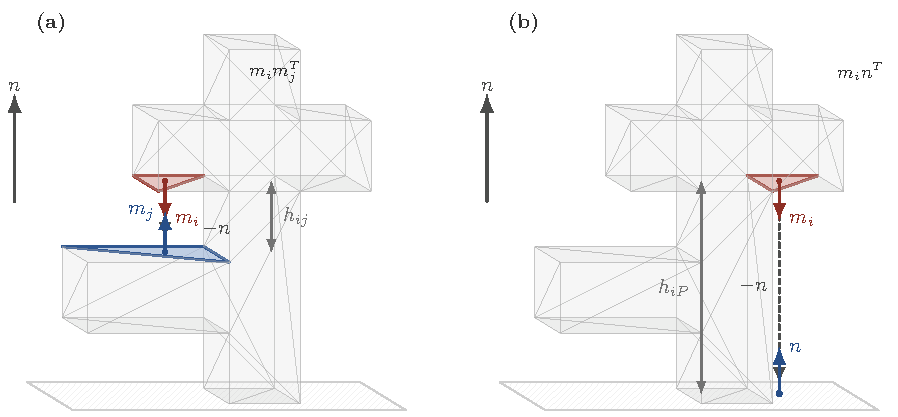
\includegraphics[width=0.9\textwidth]{pics/FTree4x_fig1_unified_flow.pdf}
\caption{Unified flow interpretation. Face-to-face support uses receiver normal $m_j$, while direct build-plate support is represented by a virtual receiver with normal $n$; the latter gives the Rayleigh contribution $B(n)$ in Eq.~\eqref{eq:Rtilde}.}
\label{fig:unified-flow}
\end{figure}

\subsection{Candidate Generation and Rescoring}

The deployed score is
\begin{equation}
J(n)=\tilde R(n)+P(n),\qquad
P(n)=\sum_{(i,j)\in\mathcal{R}(n)}O_i(n)A_iA_j,
\end{equation}
where $P$ is the face-to-face overhang amount after the height attenuation in $w_{ij}$ cancels. Because $O_i$, $w_{ij}$, and $\alpha h$ are dimensionless, $R$ and $P$ carry units of area squared while the build-plate term $B$ carries units of area: under a uniform rescaling of the mesh by a factor $s$, $R$ and $P$ scale as $s^4$ whereas $B$ scales as $s^2$, so the raw sum $J=\tilde R+P=R+P+B$ is unit-dependent and the balance among its terms shifts with model size. $J$ is therefore treated as a screening feature only, never as the final ranking criterion. A $512$-direction Fibonacci-sphere sample is first evaluated, the best directions are locally resampled in $2^\circ$--$8^\circ$ cones, and angular non-maximum suppression keeps separated candidates. To avoid treating dimensionally different quantities as directly commensurate, the final candidate order uses rank-normalized features\footnote{In this paper, rank tuning denotes fitting weights after converting each feature to its within-candidate rank; it is an empirical candidate-ranking calibration, not continuous geometric optimization.} $[J,R,P,B,H,S,\sigma_1]$, following the standard rank-transformation idea for scale-robust empirical modeling~\cite{conover1981rank}; the rank transform makes the final ordering invariant to any strictly monotone rescaling of each feature, and hence independent of the model's units. Here $H$ is the valid-hit count and $S,\sigma_1$ are singular-value features retained only for post-processing. The reported calibration uses weights $(w_J,w_R,w_P,w_B,w_H,w_S,w_1)=(0,0.731,-2.3897,2.1447,2.3109,-2.2922,1.6363)$, and cross-validation below reports the expected loss when these weights are not fit in sample. Implementation optimizations, including first-hit fallback and per-mesh cached geometry, reduced a 1k-direction evaluation of \emph{Bunny 69k} from about $15.7$ s to $1.5$ s without changing selected directions.

\section{Evaluation Protocol and Datasets}

\subsection{Datasets and Experimental Environment}
\label{sec:datasets}

The dataset consists of five groups that deliberately separate and control the two axes of \emph{shape difficulty} and \emph{mesh scale}.
A--C set the scale in the $\sim$$10^1$--$10^5$-face range and vary the difficulty axis from basic shapes to freeform organic shapes,
revealing the \emph{fixed-cost floor} of the exhaustive sweep (a cost almost independent of mesh complexity).
D--E fix the difficulty as real manufacturing parts while pushing the scale axis from $256$ faces to $1.04\times10^6$ faces,
revealing the \emph{adaptive cost} by which the SFTF candidate-evaluation cost increases adaptively to mesh complexity.
Therefore A--E is not a single size ramp, and the partial overlap of the face-count ranges of groups C and D
is the result of a design that separates and controls the two axes, not an ordering error.
\begin{itemize}
\item \textbf{A (basic shapes, 5; lower difficulty)}: cube, sphere, cylinder, cone, torus (face count $\sim$$10^1$--$10^3$).
\item \textbf{B (simple functional parts, 5; mid difficulty)}: u\_bracket, hook, c\_clamp, pipe\_elbow, hollow\_box.
\item \textbf{C (organic/freeform benchmarks, 5; upper difficulty)}: standard scan/sculpture meshes such as \emph{Bunny 69k}, \emph{Manikin 13k}, \emph{Dragon 100k}, \emph{Happy 50k}, and \emph{Lucy 50k}. The Stanford grid meshes used in \S\ref{sec:baseline} are exactly this group.
\item \textbf{D (Thingi10K set 1, 10; lower scale)}: real manufacturing parts with $256$--$88{,}106$ faces~\cite{Thingi10K}.
\item \textbf{E (Thingi10K set 2, 10; upper scale)}: large high-resolution meshes with about $5.1\times10^5$--$1.04\times10^6$ faces.
\end{itemize}
All timing experiments were run on a Windows 11 Education 64-bit workstation with an AMD Ryzen 9 9950X3D CPU
(16 cores, 32 logical threads), 125 GB RAM, and an NVIDIA GeForce RTX 5080 GPU (16 GB, driver 595.79).
The Python implementation used Python 3.12.13 with NumPy 1.26.4, SciPy 1.17.1, Trimesh 4.4.0, Matplotlib 3.11.0, and scikit-learn 1.9.0.
TOMO\_CPU and TOMO\_CUDA were called through Windows DLL interfaces, and the SFTF\_C++ implementation was built as a Windows x64 C++ DLL
using the Visual Studio 2022/MSVC toolchain with OpenMP parallelization.

\subsection{Comparison Targets and Evaluation Protocol}
\label{sec:protocol}

We first define the comparison targets and evaluation procedure used in the quantitative analyses up to \S\ref{sec:fivegroup}.
The comparison targets are as follows.

\begin{enumerate}
\item PCA-based direction
\item Existing Support Tensor eigenvector direction
\item Initial eigenvector-based concave direction
\item This study's Support Flow Tensor Field direction
\item TOMO\_CPU or commercial-slicer-based $v_{ss}$ optimal direction
\end{enumerate}

For each mesh, we generate a $v_{ss}$ contour at $1^\circ$ intervals under a critical angle of $60^\circ$,
and evaluate how close the $v_{ss}$ value at our method's top candidate directions is to the global optimum.
Even if the direction coordinates do not match exactly, if the $v_{ss}$ values are similar we regard them as optimal orientations of the same level.
Also, considering the case where the global optimum appears scattered across multiple basins,
we compare angularly separated top-$k$ basin representatives rather than simple top-$k$ grid points.
The candidate basins proposed by SFTF are re-input to TOMO\_CPU to directly measure the Mss,
and based on that measured value we mark the measured optimal and measured worst basins.
Unless otherwise stated, both the five-mesh accuracy results and the A--E implementation audit use stored $1^\circ$ TOMO\_CPU grids. Ratio statistics at $\theta_c=60^\circ$ exclude records whose TOMO global best is nonpositive, because those cases make a positive support-volume ratio ill-defined.


\section{Results and Discussion}

\subsection{Stored TOMO Grid Comparison}

The stored $1^\circ$, $\theta_c=60^\circ$ TOMO\_CPU grids were used as the accuracy reference. SFTF candidates were mapped to the nearest signed TOMO yaw--pitch cell, and ratios were computed against the global TOMO best value. Table~\ref{tab:sftf-tomo-comparison} reports the calibration-set comparison; the rank-tuned values are intentionally treated as in-sample and are evaluated again by cross-validation below.

\begin{table}[H]
\centering
\caption{Comparison of the stored TOMO\_CPU $v_{ss}$ grid with the current SFTF candidates.
Ratio is the ratio of the SFTF candidate's $v_{ss}$ to the TOMO global optimal $v_{ss}$.}
\label{tab:sftf-tomo-comparison}
\begin{tabular}{lrrrrr}
\toprule
Mesh & TOMO best & SFTF score1 & Ratio & SFTF best-of-3 & Ratio\\
\midrule
\emph{Bunny 69k} & 4440.34 & 5217.86 & 1.18 & 5217.86 & 1.18\\
\emph{Manikin 13k} & 2956.12 & 5565.56 & 1.88 & 5565.56 & 1.88\\
\emph{Dragon 100k} & 28106.97 & 37640.00 & 1.34 & 36067.25 & 1.28\\
\emph{Happy 50k} & 8512.64 & 19894.23 & 2.34 & 18592.73 & 2.18\\
\emph{Lucy 50k} & 7605.40 & 9132.08 & 1.20 & 9132.08 & 1.20\\
\bottomrule
\end{tabular}
\end{table}

Raw ranking alone is insufficient for the \emph{Happy 50k} hard case, so SFTF is used as a warm start for local TOMO verification rather than as a standalone optimizer.

\subsection{Local Verification and Adaptive Verification Escalation}
\label{sec:budget-curve}
\label{sec:ave}

The deployed metric is a budget curve: the top-$K$ SFTF candidates define $\pm10^\circ$ local windows, and the best TOMO grid value inside their union is selected. This changes the interpretation from whether the top-3 ranking alone solves the problem to whether SFTF places a small verification budget near useful TOMO basins. Table~\ref{tab:budget-curve} summarizes this budget--accuracy trade-off.

\begin{table}[H]
\centering
\caption{Budget curve of top-$K$ local TOMO verification around SFTF candidates.
The budget is the mean fraction of the $1^\circ$ TOMO grid covered by the union of local windows.}
\label{tab:budget-curve}
\begin{tabular}{rrrrrr}
\toprule
Top-$K$ & Mean ratio & Median ratio & Max ratio & Mean grid budget & Ratio $\le 2.0$\\
\midrule
3  & 1.24 & 1.07 & 1.97 & 0.87\% & 5/5\\
10 & 1.18 & 1.02 & 1.84 & 2.03\% & 5/5\\
20 & \textbf{1.14} & \textbf{1.00} & \textbf{1.66} & 3.40\% & 5/5\\
30 & 1.14 & 1.00 & 1.66 & 5.20\% & 5/5\\
\bottomrule
\end{tabular}
\end{table}

Budget-matched controls in Table~\ref{tab:budget-matched-baseline} test whether the value is the \emph{placement} of the local windows or only the amount of grid inspected. On these organic meshes a budget-matched farthest-point uniform-axis control performs on par with SFTF and is slightly better in the worst case, so the top-$20$ ranking is not a decisive advantage over simply spreading the same verification budget; a random-seed control is weaker. Section~\ref{sec:limits} shows that on the large mechanical parts of groups D--E the uniform control is in fact clearly better than SFTF, which bounds the regime in which the ranking is useful.

\begin{table}[H]
\centering
\caption{Budget-matched local TOMO controls at the per-mesh SFTF top-$20$ grid-cell budget (five organic stored meshes).
The uniform-axis control matches SFTF in the mean and is better in the worst case; the warm-start value on these meshes is therefore not the window placement.}
\label{tab:budget-matched-baseline}
\small
\begin{tabular}{lrrrrr}
\toprule
Policy & Mean & Median & Max & Budget & $\le 2.0$\\
\midrule
SFTF top-$20$ local & 1.14 & 1.00 & 1.66 & 3.40\% & 5/5\\
Uniform-axis matched & \textbf{1.08} & 1.07 & \textbf{1.17} & 3.38\% & 5/5\\
Random matched (median) & 1.36 & 1.19 & 1.86 & 3.38\% & 5/5\\
\bottomrule
\end{tabular}
\end{table}

Table~\ref{tab:ave} reports the resulting automatic escalation policy. Adaptive Verification Escalation (AVE) escalates only when ordinary top-$10$ local verification is uncertain. The trigger uses local-verification quantities only,
\begin{equation}
\begin{aligned}
\mathrm{trigger}_{\mathrm{AVE}}
&=[\eta\ge0.008]\wedge[\mathrm{edge}=1\vee g\le1.5\vee g\ge3.0],\\
\eta&=V_{ss}^{\mathrm{loc}}/V_{\mathrm{bbox}},\qquad
 g=V_{ss}^{\mathrm{seed}}/V_{ss}^{\mathrm{loc}}.
\end{aligned}
\label{eq:ave-trigger}
\end{equation}
Here $\mathrm{edge}=1$ indicates that the best local cell lies within $1^\circ$ of a window boundary; a small gain $g\le1.5$ means the window search barely improved on the seed (a plateau), while a large gain $g\ge3.0$ means it moved far (an unreliable seed). A boundary case with $g\le1.5$ is routed to deeper escalation. These thresholds were re-fit on the overflow-corrected grids; the original submission used $\eta\ge0.03$ and shallower escalation, tuned when the large parts were excluded. Escalation only expands the verified candidate set, so it can spend more budget but cannot worsen the selected verified value.

\begin{table}[H]
\centering
\caption{Adaptive Verification Escalation (AVE) from top-$10$ local TOMO verification on the five organic stored meshes.
On the corrected grids the base top-$10$ policy already keeps all five below ratio $2.0$, so the escalation only trims the mean; the case that genuinely exercises AVE is the large-mechanical-part audit of Table~\ref{tab:ave-g5}.}
\label{tab:ave}
\small
\begin{tabular}{lrrrrr}
\toprule
Policy & Expanded & Mean & Max & Budget & $\le 2.0$\\
\midrule
Top-$10$ local & 0/5 & 1.18 & 1.84 & 2.03\% & 5/5\\
AVE & 3/5 & \textbf{1.14} & \textbf{1.66} & 9.99\% & 5/5\\
\bottomrule
\end{tabular}
\end{table}

The five stored meshes are in-sample for the detector thresholds. Table~\ref{tab:ave-g5} reports the held-out cached A--E audit, which contains $21$ ratio-valid records after excluding $14$ records with nonpositive TOMO best values at $\theta_c=60^\circ$. The valid set is larger than in the original submission because a signed-volume defect in the TOMO\_CPU voxel accumulator (a $16$-bit per-column overflow) had corrupted the support volume of the high-face-count group-E meshes; with the accumulator corrected, those meshes yield positive TOMO optima and become ratio-valid. They are genuinely hard for a coarse candidate generator, so the AVE thresholds were re-fit on the corrected grids (a lower normalized-support gate, deeper escalation, and an added large-jump trigger); the SFTF candidate ranking itself is unchanged.

\begin{table}[H]
\centering
\caption{Cached five-group audit of the tiered AVE policy on ratio-valid $1^\circ$, $\theta_c=60^\circ$ TOMO\_CPU records.
The top-$10$ baseline over all ratio-valid records has mean ratio $5.10$, maximum $62.59$, mean budget $2.26\%$, and $14/21$ records below ratio $2.0$.}
\label{tab:ave-g5}
\small
\begin{tabular}{lrrrrrr}
\toprule
Group & $n$ & Expanded & Mean & Max & Budget & $\le 2.0$\\
\midrule
A & 2 & 2 & 1.03 & 1.06 & 7.59\% & 2/2\\
B & 1 & 1 & 1.10 & 1.10 & 6.97\% & 1/1\\
C & 5 & 3 & 1.14 & 1.66 & 9.99\% & 5/5\\
D & 6 & 5 & 1.03 & 1.13 & 23.58\% & 6/6\\
E & 7 & 7 & 1.26 & 1.93 & 11.30\% & 7/7\\
\midrule
All & 21 & 18 & \textbf{1.14} & \textbf{1.93} & \textbf{13.94\%} & 21/21\\
\bottomrule
\end{tabular}
\end{table}

The audit reduces the maximum ratio from $62.59$ to $1.93$ and keeps all ratio-valid records below $2.0$ with a mean budget of $13.94\%$. The budget is higher than the original submission's because AVE now escalates on the recovered group-E meshes: the escalation is what keeps them below ratio $2.0$, and the mean budget still inspects under one seventh of the $1^\circ$ grid. The single hardest case is the $1.04$M-face \emph{Group\_E2\_790253} at ratio $1.93$; its optimum basin is only partly covered even at the deepest escalation, marking the practical ceiling of coarse SFTF candidate coverage on large parts.

\subsubsection{Representative TOMO Landscapes}
Figures~\ref{fig:dragon-landscape} and~\ref{fig:happy-landscape} show the contrast between a broad-basin ordinary case and the \emph{Happy 50k} hard case. Additional \emph{Bunny 69k}, \emph{Manikin 13k}, and \emph{Lucy 50k} landscapes are provided in Supplementary Figs.~S5--S7.

\begin{figure}[H]
\centering

\includegraphics[width=0.78\linewidth]{pics/appendix_contour_dragon.pdf}
\caption{Representative TOMO\_CPU $v_{ss}$ landscape of \emph{Dragon 100k}. The global optimum forms a distinct low-cost basin, illustrating a non-hard case where coarse SFTF candidates already cover useful regions.}
\label{fig:dragon-landscape}
\end{figure}

\begin{figure}[H]
\centering

\includegraphics[width=\linewidth]{pics/appendix_contour_happy.pdf}
\caption{\emph{Happy 50k} before and after AVE on the same TOMO\_CPU $v_{ss}$ landscape (corrected grids; TOMO optimum $v_{ss}=8{,}513$). The base top-$10$ local verification lands at ratio $1.84$ and AVE improves it to $1.66$; unlike the earlier overflow-affected data, on the corrected landscape \emph{Happy 50k} is only a mild hard case, and the decisive escalation cases are the large mechanical parts of Table~\ref{tab:ave-g5}.}
\label{fig:happy-landscape}
\end{figure}

\subsection{Feature Contribution and Generalization}
\label{sec:ablation}
\label{sec:unified}
\label{sec:cv}
\label{sec:baseline}
\label{sec:robustness}

Table~\ref{tab:feature-corr} reports Spearman rank correlations over the full candidate pools and shows that the build-plate term is the most stable single predictor of TOMO $v_{ss}$.

\begin{table}[H]
\centering
\small
\caption{Spearman rank correlation between features and TOMO $v_{ss}$ over the entire candidate pool.
The larger the positive value, the more valid the feature is as a cost.}
\label{tab:feature-corr}
\begin{tabular}{lrrrrrr}
\toprule
Feature & \emph{Bunny 69k} & \emph{Manikin 13k} & \emph{Dragon 100k} & \emph{Happy 50k} & \emph{Lucy 50k} & Average\\
\midrule
$J=R{+}P{+}B$         & 0.37 & 0.35 & 0.80 & 0.33 & 0.68 & 0.51\\
$R$ (Rayleigh)        & 0.36 & $-0.35$ & $-0.56$ & 0.13 & 0.16 & $-0.05$\\
$P$ (pair flow)       & $-0.09$ & $-0.41$ & $-0.71$ & 0.10 & $-0.67$ & $-0.36$\\
$B$ (build-plate)     & \textbf{0.42} & \textbf{0.74} & \textbf{0.84} & \textbf{0.23} & \textbf{0.72} & \textbf{0.59}\\
$H$ (hit count)       & 0.24 & $-0.58$ & $-0.72$ & 0.13 & $-0.82$ & $-0.35$\\
$S$ (nuclear)         & $-0.07$ & $-0.39$ & $-0.69$ & 0.08 & $-0.29$ & $-0.27$\\
$\sigma_1$            & $-0.09$ & $-0.36$ & $-0.65$ & 0.05 & 0.07 & $-0.20$\\
\bottomrule
\end{tabular}
\end{table}

The full objective ablation is moved to Supplementary Table~S5. It shows that adding nuclear/$\sigma_1$ terms does not alter candidate selection, while tensor-only variants are weakest. Table~\ref{tab:unified-corr} then separates the unified Rayleigh term from its components. The ground-node reformulation explains why $B$ is not merely a scalar patch: the unified Rayleigh term $\tilde R=R+B$ is a tensor contraction and has the strongest average single-feature correlation.

\begin{table}[H]
\centering
\caption{Spearman correlation of the unified Rayleigh term $\tilde R=R+B$ and single terms with TOMO $v_{ss}$ (higher is better).
$\tilde R$ was computed directly from the augmented tensor and agrees with $R+B$ within $10^{-12}$.}
\label{tab:unified-corr}
\begin{tabular}{lrrrr}
\toprule
Mesh & $R$ & $B$ & $\tilde R=R{+}B$ & $J=R{+}P{+}B$\\
\midrule
\emph{Bunny 69k}   & 0.36 & 0.42 & \textbf{0.43} & 0.37\\
\emph{Manikin 13k} & $-0.35$ & 0.74 & 0.73 & 0.35\\
\emph{Dragon 100k}  & $-0.56$ & 0.84 & \textbf{0.88} & 0.80\\
\emph{Happy 50k}   & 0.13 & 0.23 & 0.29 & 0.33\\
\emph{Lucy 50k}    & 0.16 & 0.72 & 0.73 & 0.68\\
\midrule
Average    & $-0.05$ & 0.59 & \textbf{0.61} & 0.51\\
\bottomrule
\end{tabular}
\end{table}

The best-of-3 comparison in Supplementary Table~S6 shows the same trend: excluding the \emph{Happy 50k} hard case, removing the negative-signal $P$ term (from $J{=}R{+}P{+}B$ to build-plate-only $B$) improves the mean ratio from $2.00$ to $1.67$. A height-convention check also supported the current sign choice: amplification for tall build-plate support and attenuation for distant face-to-face support.

Cross-validation exposes the optimism of calibration-set rank tuning. Table~\ref{tab:lomo-cv} summarizes the leave-one-mesh-out (LOMO) check: training excludes the target mesh, fits the rank-normalized weights on the others, and evaluates the held-out best-of-3 ratio.

\begin{table}[H]
\centering
\caption{LOMO cross-validation best-of-3 ratio of rank tuning (lower is better).
The in-sample column is the calibration-set fit value reported in Table~\ref{tab:sftf-tomo-comparison}.
The oracle is the best direction existing within the candidate pool, representing the upper bound of candidate generation.}
\label{tab:lomo-cv}
\begin{tabular}{lrrrr}
\toprule
Mesh & oracle & untuned $J$ & in-sample (reported) & LOMO\\
\midrule
\emph{Bunny 69k}    & 1.02 & 1.38 & 1.21 & 1.21\\
\emph{Manikin 13k}  & 1.17 & 5.02 & 2.87 & 3.02\\
\emph{Dragon 100k}   & 1.03 & 1.40 & 1.41 & 1.41\\
\emph{Lucy 50k}     & 1.01 & 1.20 & 1.10 & 1.20\\
\midrule
Average     & 1.06 & 2.25 & \textbf{1.64} & \textbf{1.71}\\
\bottomrule
\end{tabular}
\end{table}

The in-sample average $1.64$ becomes $1.71$ under LOMO on these organic meshes, still better than PCA ($1.95$) and the symmetric Support Tensor baseline ($2.46$); \emph{Manikin 13k} is the one case where PCA ($2.90$) edges out the tuned SFTF ordering ($3.02$). Table~\ref{tab:unified} summarizes this comparison. The generalization margin is much smaller than the overflow-affected data suggested, and \S\ref{sec:limits} shows it does not hold at all on large mechanical parts. This reinforces the role of rank tuning as an organic-mesh candidate-ordering heuristic, not as the final optimizer; the reliable result is obtained when SFTF candidates are followed by local TOMO verification as in \S\ref{sec:ave}.

\begin{table}[H]
\centering
\caption{Unified comparison of existing methods and SFTF (best-of-3 signed $v_{ss}$ ratio, lower is better).
SFTF-tuned is the five-mesh LOMO estimate for rank-only candidate ordering.}
\label{tab:unified}
\begin{tabular}{lrrrrr}
\toprule
Mesh & PCA & Support Tensor & SFTF untuned & SFTF tuned (LOMO) & oracle\\
\midrule
\emph{Bunny 69k}    & 1.55 & 2.11 & 1.38 & 1.21 & 1.02\\
\emph{Manikin 13k}  & 2.90 & 2.39 & 5.02 & 3.02 & 1.17\\
\emph{Dragon 100k}   & 2.10 & 1.58 & 1.40 & 1.41 & 1.03\\
\emph{Lucy 50k}     & 1.26 & 3.76 & 1.20 & 1.20 & 1.01\\
\midrule
Average     & 1.95 & 2.46 & 2.25 & \textbf{1.71} & 1.06\\
\bottomrule
\end{tabular}
\end{table}

\subsection{Five-Group Implementation Audit}
\label{sec:fivegroup}
\label{sec:impl-compare}
\label{sec:groupE}
\label{sec:critangle}
\label{sec:kray-discussion}

The A--E audit separates shape difficulty from mesh scale.

It compares TOMO\_CPU, TOMO\_CUDA, Python SFTF, and C++ SFTF on the same $1^\circ$, $\theta_c=60^\circ$ sweep setting. The full per-mesh timing table is in Supplementary Table~S1; Table~\ref{tab:fivegroup-impl} keeps the group averages.

\begin{table}[H]
\footnotesize
\centering
\caption{Group-wise average execution time and speed ratio.
The C++ SFTF average is in ms, and the TOMO and Python SFTF averages are in seconds.
The speed ranges use the same definitions as Supplementary Table~S1:
TOMO\_CPU over Python SFTF and TOMO\_CPU over SFTF\_C++.}
\label{tab:fivegroup-impl}
\begin{tabular}{lrrrrrr}
\toprule
& \multicolumn{2}{c}{TOMO} & \multicolumn{2}{c}{SFTF} & \multicolumn{2}{c}{comparison}\\
\cmidrule(lr){2-3}\cmidrule(lr){4-5}\cmidrule(lr){6-7}
Group & CPU (s) & CUDA (s) & py (s) & C++ (ms) & CPU/py & CPU/C++\\
\midrule
A & 42.75  & 15.36  & 0.32 & 8.9    & $54.4$--$381.9\times$   & $1{,}683$--$50{,}641\times$\\
B & 42.45  & 14.94  & 0.38 & 9.3    & $58.0$--$269.0\times$   & $1{,}857$--$56{,}027\times$\\
C & 51.48  & 60.13  & 1.85 & 183.6  & $23.3$--$36.9\times$   & $192$--$854\times$\\
D & 53.58  & 112.38 & 1.97 & 124.5  & $12.8$--$128.8\times$  & $213$--$8{,}920\times$\\
E & 1400.02 & 4345.17 & 19.20 & 4457.7 & $8.3$--$123.0\times$    & $56.8$--$526.4\times$\\
\bottomrule
\end{tabular}
\end{table}

Over all $35$ meshes, Python SFTF is $8.3$--$381.9\times$ faster than TOMO\_CPU, while SFTF\_C++ is $56.8$--$56{,}027\times$ faster. TOMO\_CUDA helps on simple A/B shapes but is often slower than CPU on organic and large meshes in this environment, so the dominant gain is algorithmic: reducing the number of directions to evaluate, not merely changing the exhaustive-sweep backend. Group E confirms bounded scaling: the clipped ray budget in Eq.~\eqref{eq:kray-budget} caps per-direction ray cost at $3000$ samples, so large meshes near $10^6$ faces remain feasible. Supplementary Table~S2 gives the $R/P/B$/hit decomposition, Supplementary Table~S3 gives the critical-angle sweeps, Supplementary Fig.~S1 shows the five-group best/worst overlay, and Supplementary Figs.~S2--S4 visualize the \emph{Bunny 69k} $K_{ray}$ trade-off. These results support the intended role of SFTF: a fast, interpretable candidate generator whose outputs are verified locally by TOMO or a slicer.

\subsection{Limitations: candidate ranking does not transfer to large mechanical parts}
\label{sec:limits}

The correlation and warm-start evidence above is drawn from the organic freeform meshes (group~C), on which the tensor features predict TOMO $v_{ss}$ (build-plate term $B$ has mean Spearman $0.59$, unified $\tilde R$ has $0.61$). This does not carry over to the large mechanical parts of groups D--E. Measured over a uniform direction set, the Spearman correlation between every SFTF feature and TOMO $v_{ss}$ is near zero on those parts (for $B$, $\approx 0$ on D/E and $-0.40$ on \emph{Group\_E10}), so the tuned score carries essentially no ranking signal there and its top-$20$ candidates cluster near the $3^\circ$ non-maximum-suppression floor, covering only a narrow angular region. The optimum-covering candidate then sits deep in the pool (rank $41$--$255$, and outside the pool entirely for the $1.04$M-face \emph{Group\_E2\_790253}), which is why Adaptive Verification Escalation must spend a substantially larger budget on group~E to recover a good orientation (Table~\ref{tab:ave-g5}).

A budget-matched control makes the consequence explicit. Extending the comparison of Table~\ref{tab:budget-matched-baseline} to all $21$ ratio-valid A--E meshes at the top-$20$ budget, a farthest-point uniform-axis seeding clearly outperforms the SFTF ranking, and even a random seeding does:

\begin{table}[H]
\centering
\caption{Budget-matched local TOMO controls over the full $21$-mesh ratio-valid set (top-$20$ grid-cell budget, $\approx 4\%$ of the $1^\circ$ grid). On the large mechanical parts, spreading the same budget uniformly beats the SFTF candidate ranking.}
\label{tab:budget-matched-g5}
\small
\begin{tabular}{lrrrrr}
\toprule
Policy & Mean & Max & $\le 2.0$ & D mean & E mean\\
\midrule
SFTF top-$20$ local & 3.34 & 34.04 & 15/21 & 6.85 & 2.90\\
Uniform-axis matched & \textbf{1.20} & \textbf{2.10} & \textbf{20/21} & 1.09 & 1.44\\
Random matched (median) & 1.32 & 2.56 & 20/21 & 1.15 & 1.54\\
\bottomrule
\end{tabular}
\end{table}

We report this openly because an earlier version of this study, before a $16$-bit overflow in the TOMO\_CPU voxel accumulator was corrected, excluded all of these large parts as having nonpositive support volume; the corrected data admits them and reveals the limit. A partial explanation is that on mechanical parts the symmetric second-moment tensor $M=\sum_i A_i m_i m_i^T$ of Eq.~(1) is actually the more useful predictor: its Rayleigh quotient $n^{T}Mn$ has mean Spearman $0.51$ with $v_{ss}$ over the valid set (versus $\approx 0$ for the asymmetric score), though it, too, fails on a minority of parts and does not by itself beat uniform seeding. The practical takeaway is that SFTF is best positioned as a fast, interpretable candidate generator for organic freeform parts, and as a warm start it should be combined with, not substituted for, broad angular coverage on large mechanical geometries.

\section{Conclusion}

This study proposed a direction evaluation method that combines the Support Flow Tensor Field and a build-plate penalty for build-orientation optimization in additive manufacturing.
The eigenvector interpretation of the existing symmetric tensor is useful for shape directionality, but
it does not sufficiently reflect direction-dependent overhangs, internal visibility, and the build-plate support requirement.

The current algorithm directly computes an asymmetric Support Flow Tensor for each candidate direction, and
constructs a basic objective function $J=R+P+B$ that combines the Rayleigh support cost, the face-to-face support volume, and the build-plate penalty.
In the actual final candidate selection, it applies a rank-normalized tuning score $T$ of $J,R,P,B,H,S,\sigma_1$
to a candidate pool made by coarse spherical sampling and small-angle refined sampling,
to choose promising orientations to pass to slicer/TOMO verification.
When used this way on organic freeform parts, verifying the $\pm 10^\circ$ neighborhoods of only the top-$20$ candidates recovers a mean
support-volume ratio of $1.14$ (maximum $1.66$) while inspecting $3.40\%$ of the $1^\circ$ grid, and the
AVE automatically widens this budget only for detected hard cases (\S\ref{sec:ave}). On large mechanical parts, however, the tensor features no longer predict support volume and this ranking advantage disappears (\S\ref{sec:limits}).

The quantitative analysis (\S\ref{sec:ablation}) shows both the strengths and limitations of the method.
On the five stored meshes, cross-validated SFTF rank tuning is superior to PCA and Support Tensor eigenvector directions, supporting the starting assumption.
At the same time, the five-group $1^\circ$ nested CV shows that rank-only scoring is not sufficiently reliable as a standalone optimizer.
Most of the predictive power originates from the build-plate penalty and the internal visibility evaluation,
the marginal contribution of some tensor-derived terms such as nuclear/$\sigma_1$ is small, and
the calibrated rank tuning weights show an optimistic bias on unseen meshes.
Meanwhile, in \S\ref{sec:groundnode}--\S\ref{sec:unified} we showed that the build-plate penalty is exactly equivalent
to the Rayleigh contribution obtained by adding a virtual ground node to the flow tensor.
This unifies the term driving the predictive power into the tensor contraction $\tilde R=R+B$, justifying the ``tensor'' formulation,
and confirms that on the organic meshes $\tilde R$, excluding the negative-signal face-to-face support volume $P$, is superior to the existing $J$. As \S\ref{sec:limits} details, this predictive power is specific to organic freeform geometry and does not extend to large mechanical parts.

Therefore, in future work we will (i) determine the weights on a cross-validation basis rather than a calibration set to control overfitting,
(ii) remove terms with marginal contribution or replace them with features highly correlated with the actual $v_{ss}$,
such as face-to-face self-support coverage or a support-volume proxy,
(iii) normalize the dimensions of the objective-function terms to secure the physical meaning and transferability of the weights,
(iv) add projection-area, print-height, and contact-stability terms to extend to a multi-objective orientation optimization model, and
(v) as observed in \S\ref{sec:critangle}, since the TOMO optimal orientation shifts with the critical angle $\theta_c$ while
the current SFTF candidates are invariant to $\theta_c$, extend to $\theta_c$-dependent candidate generation with overhang truncation turned on.
For cases where the ordinary top-$K$ candidate generation does not include a stable near-optimal basin,
AVE provides an automatic escalation path, and future work will refine its thresholds on a larger family-held-out validation set.

\section*{Statements and Declarations}

\subsection*{Funding}
Funding information is provided separately in the submission system and title-page file to preserve double-anonymous review.

\subsection*{Competing interests}
The author declares no competing interests.

\subsection*{Data availability}
The numerical results reported in this manuscript are based on cached mesh-evaluation records, support-volume grids, and generated summary tables maintained with the research code.
An anonymized repository or supplementary archive can be supplied during peer review, and the permanent public repository link can be provided after acceptance.
Third-party mesh models should be obtained from their original sources subject to their respective licenses.

\subsection*{Code availability}
The code and scripts supporting the reported results will be made publicly available upon acceptance.
An anonymized review archive can be provided during peer review if required.

\subsection*{Use of artificial intelligence tools}
AI coding assistants, including OpenAI Codex and Anthropic Claude Code, were used to assist with portions of research-code implementation, figure-generation scripts, and manuscript-support automation.
All generated code, experimental results, and manuscript changes were reviewed and validated by the author.

\subsection*{Ethics approval and consent to participate}
Not applicable.

\subsection*{Consent for publication}
Not applicable.

\bibliographystyle{sn-basic}
\bibliography{references}

\end{document}
